\documentclass[11pt,wide]{mwart}

\usepackage[utf8]{inputenc}
\usepackage{polski}
\usepackage{graphicx}
\usepackage{amsmath}
\usepackage{hyperref}

\date{Wrocław, \today}
\title{\LARGE\textbf{Pracownia z analizy numerycznej}\\Pracownia P0}
\author{Mikołaj Korobczak}

\begin{document}
\maketitle
\thispagestyle{empty}
\tableofcontents

\section{Funkcja kwadratowa}
Przykładowa funkcja kwadratowa
\subsection{Wzór}
Wzór omawianej funkcji:
\begin{equation}\label{E:kwadrat}
f(x) = \frac{1}{e}(x + \frac{3x}{17})^2
\end{equation}

\subsection{Tabela}
Poniższa tabela zawiera kilka wartości omawianej funkcji \eqref{E:kwadrat}
\begin{center}

	\begin{tabular}{|c|c|} \hline
	x & f(x) \\ \hline
	-8	&	32.58724461587863174827361945062876\\
	-7	&	24.94960915903206810639858304057270\\
	-6	&	18.33032509643172858204707154072821\\
	-5	&	12.72939242807759185893701214808971\\
	-4	&	8.14681115396965793706840486265719\\
	-3	&	4.58258127410793214551176788518205\\
	-2	&	2.03670278849241448426710121566430\\
	-1	&	0.50917569712310362106677530391607\\
	0	&	0.00000000000000000000000000000000\\
	1	&	0.50917569712310362106677530391607\\
	2	&	2.03670278849241448426710121566430\\
	3	&	4.58258127410793214551176788518205\\
	4	&	8.14681115396965793706840486265719\\
	5	&	12.72939242807759185893701214808971\\
	6	&	18.33032509643172858204707154072821\\
	7	&	24.94960915903206810639858304057270\\
	8	&	32.58724461587863174827361945062876\\ \hline
	\end{tabular}
	

\end{center}

\subsection{Wykres}
Wykres funckji \eqref{E:kwadrat}: \\
\begin{figure}[ht]
	\begin{center}
	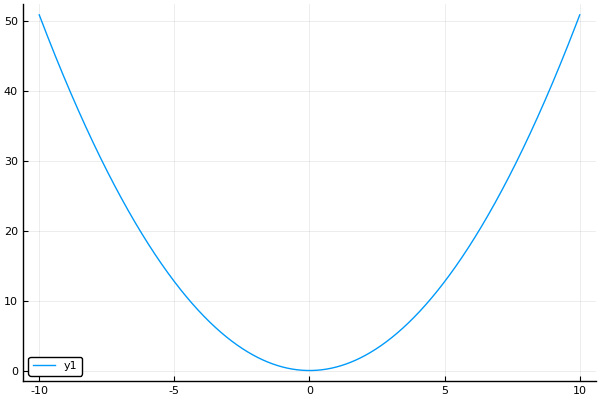
\includegraphics[width=10cm]{wykres}
	\end{center}
	\caption{Wykres z jupytera}
\end{figure}

\section{Twierdzenie Taylora (o szeregu)}

\subsection*{Wzór}
\begin{equation*}
f(x) = f(a) + \frac{x - a}{1!}f^{(1)}(a) + \frac{(x - a)^2}{2!}f^{(2)}(a) + \dots + 
\frac{(x - a)^n}{n!}f^{(n)}(a) + R_n(x, a) = \sum^n_{k=0}(\frac{(x-a)^k}{k!}f^{(k)}(a)) + R_n(x,a)
\end{equation*}

Gdzie $f^{(k)}(a)$ jest pochodną k-tego rzędu, a $R_n(x,a)$ spełnia warunek: 

\begin{equation*}
\displaystyle\lim_{n\to\infty}\frac{R_n(x,a)}{(x- a)^n} = 0
\end{equation*}

\end{document}




